\chapter{Notifikační systém}
V rámci integrace spisové služby \ref{chap:integrace-spis-sluzby} do ŠIS se ukázalo jako nezbytné navrhnout dílčí komponentu - Notifikační systém. Tato komponenta představuje klíčový prvek pro efektivizaci procesů správy dokumentů a komunikaci v rámci školy. Jeho zavedení by mělo přispět k automatizaci generování a distribuce dokumentů, zrychlení procesů a snížení administrativní zátěže na personál.

Notifikační systém by měl být koncipován tak, aby poskytoval automatické notifikace o nových či změněných dokumentech, potřebě zpracování nebo schválení, a to všem relevantním stranám. Tím by se zvýšila transparentnost administrativních procesů a zefektivnila komunikace mezi třídními učiteli, administrativními pracovníky a vedením školy.

Při návrhu notifikačního systému je důležité přistupovat s ohledem na univerzálnost a rozšiřitelnost. Systém by neměl být omezen pouze na aktuální požadavky spojené s integrací spisové služby \ref{chap:integrace-spis-sluzby}, ale měl by být koncipován tak, aby snadno zvládal budoucí rozšíření a nová využití.

Tento přístup umožní využívat notifikační systém pro širokou škálu účelů, včetně informování žáků o nových známkách, upozornění učitelů na dlouhodobě nezapsanou absenci ve třídní knize, nebo dokonce automatické připomenutí důležitých školních událostí a termínů. Taková flexibilita znamená, že nofitikační systém se může stát důležitým prvkem komunikace podporujícím širokou škálu školních procesů a interakcí.

Navrhování systému s ohledem na budoucí potřeby a možnosti rozšíření je přístup, který zajišťuje, že investice vývoje přispěje k dlouhodobé udržitelnosti a přinese novou, trvalou hodnotu.

\section{Návrh řešení}
\begin{landscape}
    \begin{figure}[H]
        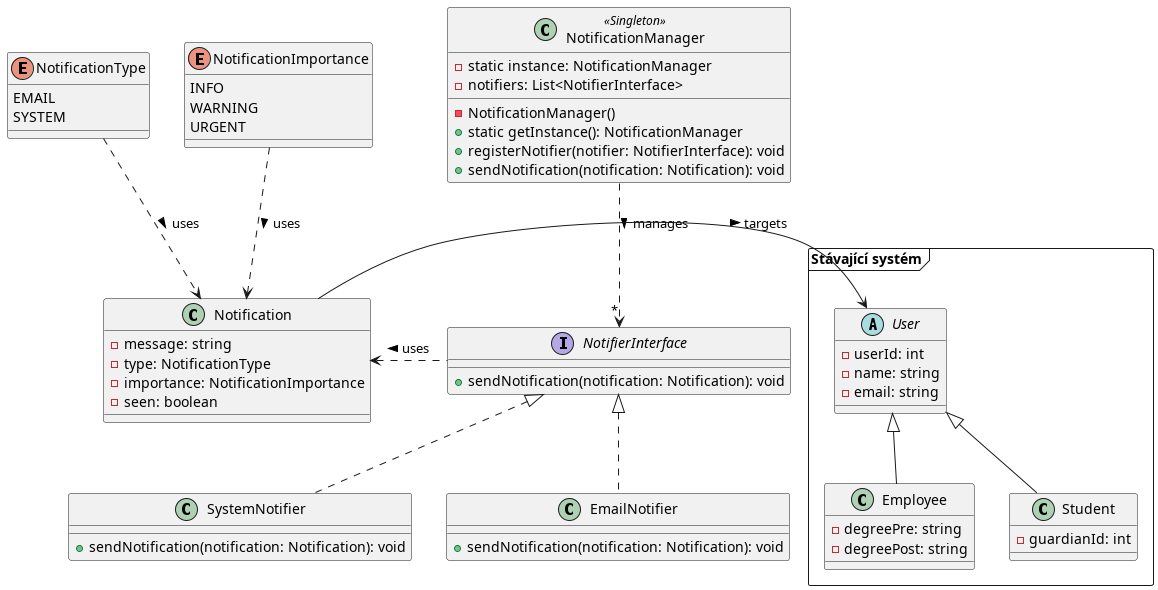
\includegraphics[width=\linewidth]{cl-notifikacni-system.png}
        \caption{Diagram tříd navrženého systému}
        \label{fig:cl-notifikacni-system}
    \end{figure}
\end{landscape}

\subsection*{Popis tříd, vztahů a návrhových vzorů}
Diagram \ref{fig:cl-notifikacni-system} zobrazuje architekturu notifikačního systému, který se skládá z několika komponent:
\begin{itemize}
    \item \textbf{NotifierInterface}: Toto rozhraní definuje základní metodu sendNotification(notification: Notification), která slouží k odesílání notifikací. Implementace tohoto rozhraní umožňuje vytvoření různých typů odesílatelů notifikací, jako jsou systémové notifikace nebo e-mailové notifikace.

    \item \textbf{Notification}: Třída reprezentuje samotnou notifikaci, obsahuje atributy jako message (text notifikace), type (typ notifikace, například EMAIL nebo SYSTEM), importance (důležitost notifikace, například INFO, WARNING, URGENT) a seen (boolean hodnota indikující, zda byla notifikace zobrazena).
    
    \item \textbf{NotificationType a NotificationImportance}: Enumerace, které definují možné typy a úrovně důležitosti notifikací. Pomocí těchto enumerací je možné jednoduše rozšířit systém o nové typy a priority notifikací.
    
    \item \textbf{User}: Abstraktní třída definující základní vlastnosti uživatelů systému, jako jsou userId, name a email. Tato třída je rozšířena třídami Employee a Student, které přidávají specifické atributy relevantní pro zaměstnance a studenty.
    
    \item \textbf{NotificationManager}: Třída, která využívá návrhový vzor Singleton, zajišťuje centralizovanou správu notifikací a jejich odesílatelů. Umožňuje registraci odesílatelů notifikací a zprostředkovává odesílání notifikací všem odesílatelům.
\end{itemize}
Návrh disponuje pouze několika atributy, které jsou, či budou reálně využívány.

Významným návrhovým vzorem použitým v tomto systému je Singleton, který je aplikován na NotificationManager k zajištění jediné instance správce notifikací v aplikaci. Tento vzor pomáhá udržovat konzistentní stav notifikací a zajišťuje, že všechny komponenty systému pracují s právě jedním objektem pro správu notifikací.
